\documentclass[12pt]{article}

% Packages
\usepackage[a4paper, margin=2.5cm]{geometry}
\usepackage{graphicx}
\usepackage{amsmath, amsthm}
\usepackage{booktabs}
\usepackage{float}
\usepackage{fancyhdr}
\usepackage{titlesec}
\usepackage{caption}
\usepackage{hyperref}
\usepackage{lmodern}
\usepackage{multirow}
\usepackage{titling}
\usepackage{pgfplotstable}
\usepackage{algorithm}
\usepackage{algpseudocode}
\usepackage{xcolor}
\usepackage{tabularx}
\usepackage{amssymb}
\usepackage{enumitem}
\usepackage[most]{tcolorbox} 
\usepackage{adjustbox}
\usepackage{pdfpages}  
\usepackage[normalem]{ulem}

\includepdfset{pagecommand=\thispagestyle{fancy}}
\tcbuselibrary{breakable} 

% Header & Footer
\pagestyle{fancy}
\fancyhf{}
\rhead{Neurosymbolic AI for Social Cognition - Literature Study}
\lhead{Jarne Demoen - 0616897}
\rfoot{\thepage}
\setlength{\headheight}{14.5pt}

% Title
\title{Neurosymbolic AI for Social Cognition - Literature Study}
\author{Jarne Demoen\\
Vrije Universiteit Brussel}
\date{29/10/2025}

% Custom subtitle (above main title)
\pretitle{%
  \begin{center}
  \large\textbf{Master's Thesis}\\[1ex]
}
\posttitle{\end{center}}

\begin{document}
\maketitle
\section{Neurosymbolic AI for Social Cognition}
This thesis aims to combine neural and symbolic AI to improve how computers understand the term "social cognition". Social cognition is the way humans interpret others' emotions, intentions, and social situations.

\begin{itemize}
	\item{\textbf{Symbolic AI} uses explicit rules such as "people are happy at weddings"}
	\item{\textbf{Subsymbolic AI (deep learning)} uses pattern recognition from raw data (facial expression in images)}
	\item{\textbf{Neurosymbolic AI} merges both terms such that neural networks can extract features while logic modules can reason over structured knowledge}
\end{itemize}

The research should determine whether symbolic knowledge improves recognition or reduces the need for more data when aiming for better performance. Additionally, it would also be interesting to find out whether the integration of symbolic knowledge enhances interpretability. I will mainly be using the FindingEmo dataset.

\section{A Circumplex Model of Affect --- James A. Russell}

Russell’s paper presents a psychological model of human emotions called the \textit{Circumplex Model of Affect}, which proposes that emotions can be organized within a two-dimensional continuous space. Affect is the broadest and most general word psychologists use for how people feel emotionally or even physically. The continuous space consists of two axes:

\begin{itemize}
    \item \textbf{Valence (Pleasure–Displeasure axis)}: how positive or negative a feeling is.
    \item \textbf{Arousal (Activation–Deactivation axis)}: how energized or calm the feeling is.
\end{itemize}

Together, these dimensions form a circular structure (\textit{circumplex}) where emotions gradually blend into one another across valence and arousal, the same way as colors on a wheel. This circular arrangement provides a structured, interpretable framework for representing affect. In the context of neurosymbolic AI, it enables \textbf{symbolic encoding of affective knowledge} (\textit{anger} = unpleasant + high arousal) that can interact with neural perception modules, thus bridging psychological theory with AI reasoning.

\vspace{1em}
\noindent
In Schlosberg’s early studies, participants categorized facial expressions of emotion. Errors in these categorizations revealed that similar emotions were frequently confused, indicating that they were \textbf{conceptually close}. From these confusion patterns, Schlosberg proposed a circular representation based on two bipolar dimensions:
\begin{itemize}
    \item Pleasantness–Unpleasantness
    \item Attention–Rejection (or Activation–Deactivation)
\end{itemize}
Emotions, therefore, are better understood as positions along \textbf{continuous bipolar scales} rather than discrete, isolated categories. If one feels happy, one cannot simultaneously feel sad; if one feels tense, one cannot feel relaxed. Russell extended this reasoning, showing that any emotion word can be represented as a specific blend of valence and arousal, producing a full circle of affective experience.

\begin{figure}[H]
    \centering
    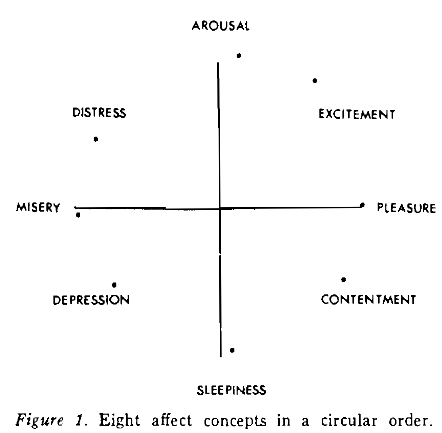
\includegraphics[width=0.9\textwidth]{Media/affect8circle.png}
\end{figure}

\vspace{1em}
\noindent
Russell’s experiment involved participants judging the relationships among the 28 emotion words. These served as the “points” later positioned within affective space using three techniques:
\begin{itemize}
    \item \textbf{Ross' circular ordering:} Arranges variables along a circle, assuming circularity from the start.
    \item \textbf{Multidimensional scaling (MDS):} Derives spatial relationships purely from perceived similarity, without assuming circularity.
    \item \textbf{Unidimensional scaling:} Rates each term separately on pleasure–displeasure and arousal dimensions, producing two coordinates per emotion.
\end{itemize}

All three approaches yielded \textbf{remarkably consistent results}. Participants did not treat emotions as independent categories. Instead, emotion words such as \textit{happy}, \textit{excited}, and \textit{content} had overlapping meanings, a property Russell called \textbf{fuzziness}. This fuzziness explains why affective terms distribute smoothly around a circle: emotions gradually blend into one another rather than having sharp boundaries. Participants’ high consistency in word placement confirmed that people share a similar \textbf{mental map of emotions} structured around the valence and arousal dimensions.

\begin{figure}[H]
    \centering
    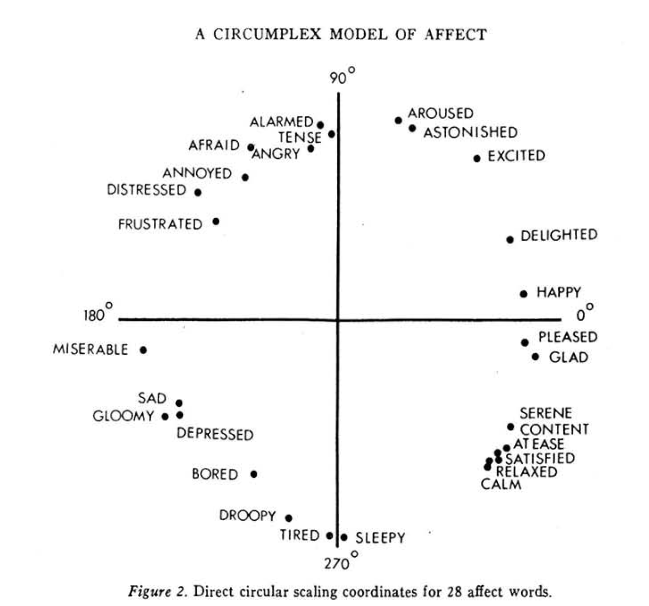
\includegraphics[width=0.9\textwidth]{Media/affect28circle.png}
\end{figure}

\noindent
Russell’s results supported three major hypotheses about the cognitive structure of affect:
\begin{itemize}
    \item \textbf{Bipolarity:} Opposite emotions (e.g., happiness–sadness) occur approximately 180° apart.
    \item \textbf{Two interpretable dimensions:} The horizontal and vertical axes correspond to pleasure–displeasure and arousal–sleepiness.
    \item \textbf{Continuity:} Rather than forming distinct clusters, emotion words spread continuously around the circle, creating a smooth emotional spectrum.
\end{itemize}

Earlier psychological models described emotions as 6–12 independent categories. Russell demonstrated instead that affective experience is \textbf{interconnected and continuous}, characterized by two bipolar dimensions that explain most of the variance in emotional life.

\bigskip
\noindent
\textbf{From feeling to cognition:}  
Russell compared two types of emotion data: self-reports (how people feel) and judgment data (how people think about emotion terms). Traditionally, self-reports were believed to reveal genuine emotional experience, while judgment data were thought to capture only linguistic or semantic relationships. Yet, both data types yielded the same circular structure. This finding implies that \textbf{the way people experience emotions and the way they conceptualize them share the same underlying mental framework}.

\medskip
\noindent
Emotions are therefore not raw sensations; they are \textbf{interpreted experiences}.
From a neurosymbolic perspective, this implies that the \textbf{symbolic layer of an AI system} can use this cognitive map as a structured knowledge base for affective reasoning. Neural networks may handle perception (detecting facial or scene context cues), while the symbolic layer interprets these signals within the valence–arousal framework, mirroring how humans conceptualize affect.

\end{document}